\chapter{Literature Review}
\label{ch:literature_review}


This chapter establishes why end-of-life (EoL) reverse osmosis (RO) membranes are worth recovering rather than discarding, then narrows to the two things that determine whether polyamide regeneration can work in practice: the condition of the polysulfone substrate it is built on, and the fouling layer that must be removed before a new film can form.
% Write LAST. Max 100 words.


% =====================================================================
\section{The end-of-life RO membrane problem}
\label{sec:eol-problem}
\label{sec:eol-routes}

Reverse osmosis (RO) has emerged as the dominant desalination technology in desalination plants operational worldwide, and as of 2019, 15,906 desalination plants worldwide collectively produce around 95 million $\mathrm{m^3}$ of water per day \citep{Jones2019}. Despite attempts to improve service life, in most desalination applications RO membranes typically remain in service for five to nine years \citep{Ding_2026, Lawler2015}. It is estimated that 5--20\% of membranes are replaced annually \citep{BerattoRamos2024, imdea2018transfomem, Guclu2022}, translating to a huge amount of polymeric waste. Increased global RO development and increasing water demands drive more membrane usage and waste. The lack of a viable recycling infrastructure makes EoL membranes a fast-growing solid waste issue associated with water treatment.

Existing waste disposal techniques employed for EoL membranes currently mainly include landfill and incineration \citep{Khanzada2024}. Because the module is almost entirely polymeric (polyester (PET), polysulfone (PSf), polyamide (PA) and polypropylene), it is classified as an inert municipal solid waste, and the material only degrades approximately 1--5\% over 100 years \citep{Lawler2015}. In land-constrained countries such as Japan and Singapore, incineration is used instead \citep{Lawler2015}. Incineration reduces the waste volume and partly recovers the thermal energy, but the combustion of the polymers can release a range of harmful gases including NO$_x$ and SO$_2$. Incineration produces a higher CO$_2$-equivalent emission than any reuse or recycling route \citep{Lawler2015}.

Both routes discard the element completely while it still holds recoverable value. An EoL membrane element retains most of the structural integrity of its PET and PSf support \citep{Molinaa2018}. Directly reusing an EoL membrane offsets around 33\% of the environmental impact of manufacturing a replacement \citep{Lawler2015}. The alternatives to disposal do not recover the value of a working RO membrane and permanently remove its high selectivity. This chapter aims to question whether the functionality of EoL RO membranes can be restored by replacing the PA layer on the recovered support, recovering the value of the PET and PSf while uplifting its selectivity \citep{Ogbe2025,Ogbe2026}.


\subsection{Reuse and material recovery}
\label{sec:reuse}
Direct reuse moves an EoL membrane element to operating conditions with milder salinity and pressure (usually an earlier stage within the same plant) \citep{Lawler2015}. It is the most environmentally favourable option reviewed, offsetting about 33\% of the impact of a new module \citep{Lawler2015}, but it restores no function and only defers disposal by one cycle. Research by \cite{Guclu2022} has also looked into a solvent-based recycling of the thing-film composite (TFC) sheet itself, by immersing membrane pieces into dimethyle formamide. This process can delaminate the three layers, disolving the PSf layer while PET and PA stays solid. Then, NaOCl is applied to strip the remianing PA. Both PET and PSf were recovered in high purity, and the recovered PSf had a molecular weight comparable to commercial pristine PSf, so it could potentialyl replace virgin polymer in new membranes \citep{Guclu2022}. The cross-linked PA however could not be reused beyond filler or incineration feed, and the paper only demonstrated the process on small, freshly cut scales excluding fouling and contaminantes that real EoL elements can carry.  

\subsection{Chemical downcycling to NF and UF}
\label{sec:downcycling}
The most studied recycling route for EoL RO membranes uses the PA's susceptibility to oxidation, while the PSf retains its integrity \citep{GarciaPacheco2015,Molinaa2018}. With controlled NaOCl exposure, EoL membranes can be converted to nanofiltration (NF) and then ultrafiltration (UF) range performance \citep{GarciaPacheco2015}. UF membranes made from brackish water elements showed a higher permeability than those from seawater elements, suggesting brackish water membranes are a better candidate for conversion \citep{GarciaPacheco2015}. This method, however, is also sensitive to membrane fouling, as heavily biofouled membranes tend to resist NaOCl \citep{Molinaa2018}.

\subsection{Why current routes are insufficient}
None of the existing routes restores the membrane's separation ability or treats the PA layer as recoverable. Landfill and incineration destroy the element entirely; direct reuse defers rather than solves the disposal problem; material recovery returns only the thermoplastic components; and chemical conversion removes the PA layer completely. Conversion is also one-way: once the membrane is downgraded, the element can only serve as a UF or NF membrane. The proposed method aims to restore RO-grade separation on the recovered substrate \citep{Ogbe2026,Ogbe2025}.

% =====================================================================
\section{Thin-film composite RO membranes}
\label{sec:tfc-anatomy}

Thin-film composite (TFC) polyamide membranes account for the vast majority of installed RO capacity \citep{Geise2010}. They consist of three layers, each with a distinct function (Figure~\ref{fig:tfc-cross-section}):
\begin{itemize}
    \item \textbf{PET non-woven backing} ($\sim$120--150\,$\mu$m) \citep{LejarazuLarranaga2022}: provides mechanical strength to withstand operating pressures. It is the most porous and least hydraulically resistant layer, and makes up the largest mass fraction of the sheet, but contributes nothing to separation \citep{Lawler2015}.
    \item \textbf{Polysulfone (PSf) support} ($\sim$40--60\,$\mu$m) \citep{LejarazuLarranaga2022}: an asymmetric layer formed by non-solvent induced phase separation, with a finely porous skin ($\sim$10--20\,nm pores). It provides a smooth surface on which the PA layer is formed. It does not significantly increase hydraulic resistance \citep{Petersen1993}.
    \item \textbf{Polyamide (PA) selective layer} ($\sim$0.1--0.2\,$\mu$m) \citep{LejarazuLarranaga2022}: a highly cross-linked aromatic polyamide formed by interfacial polymerisation of m-phenylenediamine (MPD) in the aqueous phase and trimesoyl chloride (TMC) in an immiscible organic solvent such as hexane. The PA layer is solely responsible for salt rejection.
\end{itemize}
Because the PA layer is only nanometres thick and susceptible to chlorine attack and irreversible fouling, it is typically where most damage is found in EoL membranes. The PSf and PET layers of an end-of-life membrane often remain structurally intact, which is what makes regenerating the selective layer on the existing support feasible.


\begin{figure}[htbp]
  \centering
  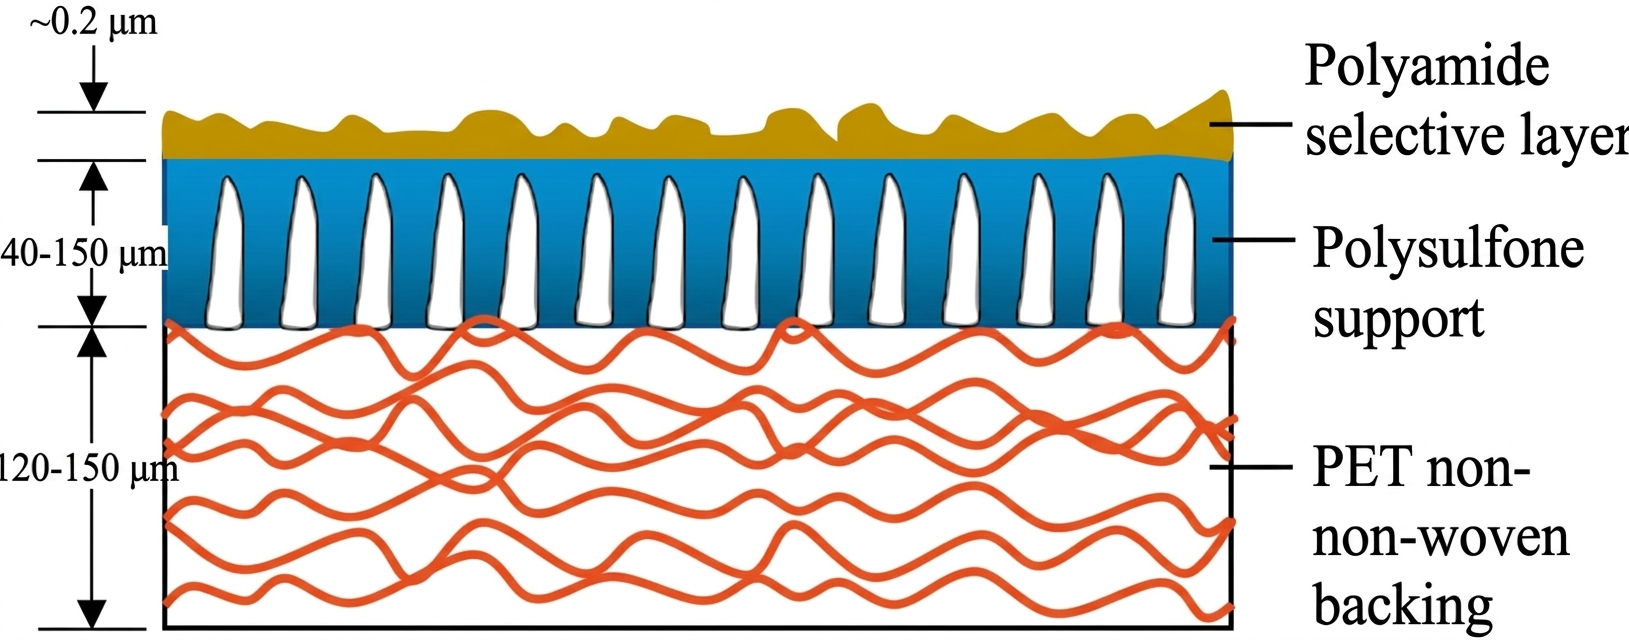
\includegraphics[width=0.8\textwidth]{figures/tfc_cross_section.jpg}
  \caption{Cross-section of a TFC RO membrane. Adapted from \citep{TFC_Composite_fig2020}}
  \label{fig:tfc-cross-section}
\end{figure}

Because the selectivity is largely concentrated in the PA layer, and the PA layer is the main site of chemical attack and fouling, regeneration aims to target the PA layer while preserving the PSf and PET beneath it.


\subsection{Polyamide Formation by Interfacial Polymerisation}
\label{sec:lit-ip}

The PA layer is formed by interfacial polymerisation (IP) \citep{Petersen1993, Nunes2020}. The porous PSf support is soaked in an aqueous solution of m-phenylenediamine (MPD). Excess solution is removed and trimesoyl chloride (TMC) is dissolved in an immiscible organic solution (typically n-hexane) and passed over the membrane support \citep{Wang2026,GhoshHoek2009}. The N--H groups of MPD react with the acyl chloride groups in TMC via nucleophillic acyl substitution, releasing HCl and builds a cross linked aromatic PA layer \citep{Wang2026,Farahbakhsh2024}.

The TMC can dissolve in n-hexane but is insoluble in water \citep{Wang2026}. MPD diffuses out of wetted pores in the PSf and into the organic n-hexane solution \citep{GhoshHoek2009}. As a result, the film grows on the surface of the PSf layer. The solubility and diffusivity of MPD therefore have a strong effect on polymerisation \citep{GhoshHoek2009}. The reaction is also much faster than the speed of monomer diffusion, so PA formation is controlled by the supply of MPD rather than reaction time. It is therefore important to optimise the crossflow velocity, pump speed and concentration to adjust the thickness of the film. Initial film also slows further monomer diffusion, creating a self-limiting reaction \citep{Wang2026,Chen2024}. 

The properties of the PA depend on the monomer structure, concentration, solvent choice, reaction time, temperature and curing conditions, as well as the surface it forms on (Section~\ref{sec:substrate}) \citep{GhoshHoek2009}. With a more linked film, higher rejection and lower flux can be expected as less crosslinking can cause larger pores and higher permeability \citep{Chen2024}.

The choice of monomers also play a key role in the film developed from IP. Conventional RO membranes are usually made from MPD/TMC, and NF membranes from piperazine (PIP)/TMC \citep{Chen2024}. PIP tends to form a relatively linear, less densely crosslinked layer with a higher water permeance and lower salt rejection compared to that of MPD, making it suited to NF \citep{Wang2026}. MPD is an aromatic diamine and TMC has three acyl chloride groups, reacting to form a three-dimentional crosslinked network \citep{Wang2026}. MPD reacts rapidly with TMC to give a highly crosslinked aromatic PA that has high salt rejection and good water permeability \citep{Wang2026}. These MPD/TMC layers created in labs commonly reach high NaCl, with \citet{Huang2022} reporting 99.0\% $\pm$ 0.4\%. This pair of chemical has been common for RO manufacturing since FT-30 membrane in 1978 and is still used widely \citep{Wang2026}. A PA layer regenerated with MPD/TMC therefore aims to match the original layer of most commercial RO membranes. 


\subsection{The Polysulfone Substrate and Effect on Film Formation}
\label{sec:substrate}

IP happens on the PSf surface, and the PSf plays an active role in film formation. The pore size, distribution, porosity and surface chemistry of the PSf strongly affect the resulting PA structure \citep{Singh2006}. The support affects how the PA forms and the path water takes through the membrane. \citet{GhoshHoek2009} showed that the amount of polyamide formed was about the same on every support they tested, but the support layer changed the location of this formation. On hydrophobic supports, more PA formed above the pores, giving thicker, rougher and more permeable films. On hydrophillic supports, more of the PA formed inside the pores, giving less permeable membranes. 

\textbf{Pore size and surface porosity.}
The pores of PSf acts as reservoir for the MPD solution. Larger pores can store more MPD, which allow more monomers to diffuse out and react with TMC during IP. If the large pores are also hydrophillic, the reaction can take place inside the pores. Larger support pores also tend to give higher salt permeability through the PA \citep{GhoshHoek2009}. Very small pores restrict the release of MPD \citep{Huang2022}. \flag{finish}

\flag{EoL membranes however can come with oxidative damage and aging, which can enlarge the pores. This presents a real issue }


\textbf{Wetting and MPD retention.}
The wettability of the support layer controls how evenly the MPD solution is spread across membranes, and how much is held. Hydrophillic pores can store more solution, which makes more available during IP \citep{Huang2022}. Highly hydrophobic supports cannot hold the solution as well. \citet{Huang2022} could not form a pristine PA layer on polyetheylene because the MPD was not retained in its pores. However, a more hydrophillic support can also release MPD slower \citep{GhoshHoek2009}. This can allow TMC to diffuse into the pores and form PA deep inside them, lowering the expected flux of the final membrane. In EoL membranes, aged PA surface can often be more hydrophillic due to additional --COOH groups from hydrolysis during operation, and cleaning chemicals used during operational lifespan can alter surface wettability. 

\textbf{Surface chemistry.}
Functional groups on the support surface can also interact with the monomers during IP. Plasma treatments can add --COOH, --CN, or --\ce{NH2} groups onto the PSf increasing its hydrophillicity, and has been reported to improve both flux and rejection of PA formed on it. Polar groups in the PSf can also hold onto MPD and slowing its release \citep{GhoshHoek2009}. Any amide groups left on the aged PA could react with TMC or MPD \citep{Farahbakhsh2024}, potentially bonding the new layer to the old one.

\textbf{Roughness and adhesion.}
\flag{Support roughness affects the final PA morphology. \citet{GhoshHoek2009} found that pure PSf supports were about twice as rough as hydrophilic blended supports ($\sim$10--11~nm vs $\sim$5--6~nm). The PA on the pure PSf had a ridge-and-valley morphology, while the PA on the blends was more nodular. The water permeability of the PA membranes also correlated strongly with support roughness \citep{GhoshHoek2009}. On stripped end-of-life membranes, \citet{Ogbe} reported roughness falling to $\sim$3.5~nm on the bare PSf and rising to $\sim$67~nm after IP. % TODO: check against Ogbe
Adhesion between the PA and the support is just as important. During IP, the growing polymer penetrates into the porous support and locks into it mechanically, which gives strong adhesion and mechanical strength \citep{Wang2026}. Weak adhesion can lead to delamination and poor long-term stability. % TODO: citation needed
This is a key risk for regeneration, as it is unclear whether a new PA layer bonds better to the old PA or to partially fouled PSf, and there is little literature on this.}


% =====================================================================
\section{Ageing and fouling of RO membranes}
\label{sec:degradation}

\subsection{Chemical and mechanical degradation}
The PA layer is very vulnerable to oxidation by sodium hypochlorite (NaOCl), mainly present during chemical cleaning. Chlorine binds to the amide nitrogen and to the adjacent aromatic ring, with bound chlorine increasing with concentration and decreasing pH \citep{Kwon2006a}. Continued attack cleaves the amide bonds and produces chain scission that breaks down the crosslinked network \citep{Kwon2006a}, so permeability rises and rejection falls. The state of the PA in EoL elements is therefore heavily affected by its cleaning history.

Mechanical ageing also acts on the support. In brackish and seawater RO operation, pressures are usually 15--70\,bar \citep{Greenlee2009}, and sustained pressure compacts the asymmetric PSf. This lowers the permeability and raises the hydraulic resistance \citep{Molinaa2018}. Improper storage and exposure to UV can also cause further physical and chemical changes to membranes \citep{Ogbe2025}. Regeneration or uplifting only replaces the PA layer, and damage to the PSf and PET cannot be undone. This sets a limit on the performance that can be recovered via IP.

The mechanism that degrades a membrane is the same mechanism used to strip the existing PA layer for IP in Section~\ref{sec:pa-removal}.

\subsection{Fouling classes and the fouling--cleaning cycle}
Fouling is one of the key reasons that RO membranes are retired \citep{GarciaPacheco2015}. There are four main classes of fouling: \textbf{organic} fouling by natural organic matter, proteins and polysaccharides; \textbf{inorganic scaling} by CaCO$_3$, CaSO$_4$, silicates and metal oxides; \textbf{particulate} fouling; and \textbf{biofouling}, in which microbial biofilms alter surface hydrophobicity and chemical composition \citep{MohiuddinAhmed2010}. \flag{humics specifically, clays, and Fe/Al/Mn oxides as colloidal
foulants, autopsy report}.

As performance declines, plants raise applied pressure and chemical concentration to maintain the same output, further shortening membrane lifespan. Oxidative damage and chlorination-induced scission increase the surface hydrophilicity and alter pore geometry, changing the fouling behaviour of the membrane \citep{Molinaa2018,Kwon2006a}.


% =====================================================================
\section{Polyamide regeneration}
\label{sec:uplifting}

\subsection{Concept and prior work}
\label{sec:uplifting-concept}
Chemical modification for recycling membranes is a recent research area as an alternative to downcycline, and utilises the PA layer's low tolerance to chlorine attacks \citep{GarciaPacheco2015}. \citet{Ogbe2025} defines uplifting as the regeneration of a degraded PA layer by IP, in which a new selective layer is formed on a chemically damaged or stripped EoL membrane. The remaining PA is first deliberatly oxidised with NaOCl to leave an intact support layer that a new PA layer can be formed on.

Uplifting restored part of the selectivity, but not to the level of a new membrane. BW30 converted at \qty{300000}{ppm.h} had a pure water permeability of \qty{93.1}{\litre\per\square\metre\per\hour\per\bar} and \qty{10.2}{\percent} NaCl rejection. After uplifting, it had \qty{11.2}{\litre\per\square\metre\per\hour\per\bar} and \qty{44.7}{\percent} \citep{Ogbe2025}. This places uplifted membrane in the NF range, and places the goal of uplifting as reinstating these membranes in lower-pressure areas such as tertiary wastewater treatment rather than RO duty \citep{Ogbe2025}. In experiments conducted by \citet{Ogbe2025}, the two EoL elements used to study conversion came from commercial membranes converted with NaOCl. Conversion also removes the fouling layer entirely, so uplifting has so far been demonstrated on clean, stripped surfaces. 

\flag{potentially insert table}



\subsection{Stripping the polyamide without destroying the substrate}
\label{sec:pa-removal}

\citet{GarciaPacheco2015} exposed EoL membranes to NaOCl, N-methyl-2-pyrrolidone (NMP) and acetone. Only NaOCl cause significant change, wehre permeability rose about \qty{385}{\percent} after \qty{20}{hr} and \qty{827}{\percent} after \qty{92}{hr}, while NMP and acetone had little effect. In this paper's review of earlier work, KMnO$_4$ had been reported as the more effective reagent when clorine doses were low, however this KMnO$_4$ gave lower permeability than high-dose NaOCl. 
In water, NaOCl forms HOCl and OCl$^-$. At pH 3, permeability changed by less than \qty{30}{\percent} over \qty{36}{hr}. After \qty{50}{hr}, permeability had risen 3.6-fold at pH 7 and 11.7-fold at pH 10.5 \citep{GarciaPacheco2015}. The authors attribute this to OCl$^-$, which makes up nearly all of the free chlorine above pH 10 but only about \qty{22}{\percent} at pH 7.
\citet{Molinaa2018} also compared \qty{50000}{ppm.h} (\qty{124}{ppm} for \qty{410}{hr}) with \qty{300000}{ppm.h} (\qty{6200}{ppm} for \qty{48}{hr}) on six EoL elements. In general, both doses gave similar permeability. FTIR showed no signs of PSf oxidation, and the roughness was compaarable to commercial PSf UF membranes. 

The dose therefore has to be high enough to remove the PA, including PA shielded by persistent foulant, but low enough not to enlarge the PSf pores. Whatever surface remains is the starting substrate for IP.

\subsection{Re-forming polyamide on a recovered substrate}
Ogbe et al.\ \citep{Ogbe2025} formed the new layer ex situ. Aqueous PIP was held on the converted surface for \qty{3}{min}, and the excess was rolled off. TMC (\qty{0.1}{wt\percent} in $n$-hexane) was then applied for \qty{60}{\second}, and the membrane was cured at \qty{60}{\celsius} for \qty{5}{min}. The PIP concentration was optimised on a new commercial PES support. Raising PIP from \qty{0.5}{wt\percent} to \qty{2.0}{wt\percent} increased MgSO$_4$ rejection from \qty{96.5}{\percent} to \qty{99.3}{\percent} and lowered permeance from \qty{29.8}{\litre\per\square\metre\per\hour\per\bar} to \qty{12.8}{\litre\per\square\metre\per\hour\per\bar}, and \qty{1.5}{wt\percent} was selected \citep{Ogbe2025}.

\iffalse
The same recipe produced a different film on converted EoL-type substrates. NaOCl leaves the surface with more carboxylic groups and a different polarity, which changes how the amine sorbs and diffuses before reaction \citep{Ogbe2025}. The result was a thinner, less crosslinked layer of irregular nodules, attributed to uneven nucleation on the altered surface. After uplifting, the amide C=O band returned at \qty{1624}{\per\centi\metre} (\qty{1663}{\per\centi\metre} on the new membrane). XPS showed that C--N and N--H bonds were restored, but the amide (O=C--N) content stayed below that of the new membrane. Roughness rose above the new membrane's (Rq \qty{67.3}{\nano\metre} against \qty{49.7}{\nano\metre}). The surface was also less negatively charged (\qty{-20.2}{\milli\volt} against \qty{-32.1}{\milli\volt}), shifting separation from RO-type transport towards NF-type steric and charge exclusion \citep{Ogbe2025}. The condition of the substrate therefore carries through into the regenerated film.

Ogbe et al.\ \citep{Ogbe2026} then developed in-situ IP, in which the monomers are dosed through a crossflow cell. They used MPD/TMC, the aromatic chemistry of RO-grade membranes, and varied monomer concentration, contact time and crossflow velocity.
\flag{Add in-situ results from Ogbe2026, and the \qtyrange{10}{60}{\second} growth-regime point already in the commented-out text of Section~\ref{sec:lit-ip}.}

Two limits remain. Rejection was stable over two \qty{3}{hr} runs, but longer-term durability under fouling and cleaning has not been tested \citep{Ogbe2025}. More importantly, IP recipes are optimised on new supports, and uplifting has been demonstrated only on surfaces stripped of both PA and foulant. Whether a cleaned, fouled substrate behaves the same way is the subject of Section~\ref{sec:fouling-ip}.
\flag{Defects as a cause of rejection variance - find a source, or move this point to Section~\ref{sec:fouling-ip}.}
\fi


% =====================================================================
\section{The Effects of Fouling on Uplifting}
\label{sec:fouling-ip}
Establishes what survives cleaning and why residual foulants are expected to disrupt interfacial polymerisation, which is the central mechanistic argument of this thesis.

\subsection{Chemical cleaning}
\label{sec:lit-cleaning}
\flag{Chemical cleaning is used to restore the flux and rejection lost to fouling. Because EoL membranes usually carry several fouling types at once, and each is removed by a different chemistry, cleaning is normally carried out in sequence with more than one agent \citep{DuPont2026}.}

Alkaline cleaning targets organic and biological foulants. At high pH, the carboxylic and phenolic groups of organic foulants deprotonate, so the foulant layer swells, becomes more negatively charged, and is more easily dispersed \citep{Ang2006}. Divalent cations such as calcium can bridge these groups and hold the foulant layer together, which limits the effect of caustic alone. Chelating agents such as EDTA bind the calcium and break these bridges, and are considerably more effective than NaOH alone for calcium-complexed organic fouling \citep{Ang2006, elimelech2005chemical}. Acid cleaning, typically with HCl or citric acid, then dissolves carbonate and phosphate scales and some metal oxides, and is generally applied after the alkaline step \citep{DuPont2026}.

Routine cleaning in plants typically lasts about an hour, whereas overnight soaks are recommended for severe or long-established fouling \citep{DuPont2026}. Even under extended conditions, some foulants are not expected to be removed. Silica particles and sand are not dissolved by acid or caustic, and iron oxides often need specialised reducing or chelating cleaners \flag{cite}. Mature biofilm extracellular polymeric substances (EPS) can also persist after cleaning \flag{cite}.

Extended exposure also affects the membrane itself, not just the foulant. \cite{tu2015chemical} soaked virgin RO membranes for \qty{25}{hr} to represent about three years of cumulative cleaning. Caustic exposure increased PWP by about \qty{5}{\percent}, acid exposure decreased it by more than \qty{10}{\percent}, and EDTA increased it by about \qty{15}{\percent}. Rejection fell by up to \qty{10}{\percent}, and these losses were mostly not recovered by a subsequent clean at the opposite pH. \cite{fujioka2014nitrosamine} similarly found that caustic exposure increased permeability and reduced conductivity rejection. Because chemical exposure alone can shift PWP this much, recovery of PWP is not a reliable measure of how much foulant a clean has removed \citep{tu2015chemical}. For regeneration, this means a cleaned EoL substrate may differ from both its fouled state and a new membrane, in both its residual foulant and its polyamide.
% ~300 words.


\subsection{Residual foulants as a barrier to interfacial polymerisation}
How material left on the substrate is expected to disrupt PA film formation.
1. Physical masking - foulant blocks the reaction interface
2. Altered wetting - hydrophobic residue can reduce MPD contact; hydrophilic residue retains water and dilutes the surface
3. Pore blockage - blocked PSf pores remove local MPD, preventing film growth
4. Chemical interference
5. Adhesion failure - PA formed on foulant rather than PSf or old PA is unsupported and delaminates under compaction.

- Defects can drive low rejections, high permeability and high replicate variance from varying fouling profiles.
- After foulants are removed, the substrate may still not behave like new PSf.
% ~400 words - the single most important block in the chapter.


\subsection{Membrane Pre-treatment for Uplifting}
\label{sec:substrate-prep}
Currently, IP is only done on clean or stripped RO membranes where the PA is almost entirely removed from the surface of the membrane. This thesis addresses whether this is necessary to prepare an EoL substrate for IP. \flag{On one hand}, if residual foulants disrupt IP by the mechanisms described above, an unclean substrate should produce a defective film. Fouling alters how EoL membranes respond to chemical treatment \citep{GarciaPacheco2015,Molinaa2018}, and fouling conditions also vary widely across different sites and applications \citep{Molinaa2018}.

Uplifting via IP on NaOCl-treated TFC membranes has shown promise in restoring EoL membrane performance \citep{Ogbe2025,Ogbe2026}, but it is not known whether removing the initial PA layer is necessary to produce a pristine PSf layer, or even whether cleaning protocols achieve this. Pre-treatment of EoL RO membranes with NaOCl introduces an extra step that membrane operation sites have to conduct in order to uplift EoL membranes, which deters the method from truly gaining widespread adoption.


\subsection{Characterising fouling profiles}
Reviews the analytical methods used to identify and quantify fouling, justifying the techniques in Section~\ref{sec:fouling-characterisation}.
- ATR-FTIR (organic groups, amide bands, PSf)
- SEM-EDS (morphology + Ca, Si, Fe, S mapping)
- XPS surface composition (confirm PA formation)
- LC-OCD and SMS (fouling characterisation)

% ~200 words, or ~120 words plus a small table.


% =====================================================================
\section{Membrane Performance Characterisation}
\label{sec:Performance-Characterisation}
Water and salt transport through the PA layer is commonly described by the solution-diffusion model \flag{ (Lonsdale 1965?)}. In this model, each species dissolves into the membrane and diffuses across under its own chemical potential gradient, and as such water and salt cross the membrane by independent mechanisms. This underpins the performance metrics used in this thesis.

\subsection{Water flux and Water Permeability}
The water flux, $J_w$, is the volumetric permeate flow per unit membrane area and is proportional to the effective pressure driving force:
\begin{equation}
  J_w = \frac{P_w}{l}\,(\Delta P - \Delta\pi) = A\,(\Delta P - \Delta\pi)
    \label{eq:water-flux}
\end{equation}
where $\Delta P$ is the applied transmembrane pressure, and $\Delta\pi$ is the osmotic pressure difference between the feed and permeate at the membrane surface. The group $P_w/l$ is the pure water permeability constant $A$. Flux in this thesis is reported as L\,m$^{-2}$\,h$^{-1}$ (LMH) and $A$ in LMH\,bar$^{-1}$. With a pure water
feed, $\Delta\pi = 0$, and $A$ is obtained directly as the pure water
permeability (PWP).

\subsection{Solute flux and solute permeability}
The solute flux is driven by the concentration difference across the barrier layer (PA):
\begin{equation}
  J_s = \frac{P_s}{l}\,(c'_W - c'') = B\,(c'_W - c'')
  \label{eq:salt-flux}
\end{equation}


% =====================================================================
\section{Research gaps and how this thesis responds}
\label{sec:research-gap}

Polyamide regeneration can recover some parts of the selectivity lost by EoL membranes, but the existing studies leave three gaps.

Gap 1: regeneration has only been demonstrated on clean, stripped substrates. In existing uplifting work, the new PA layer was formed on new commercial membranes after NaOCl conversion, which removes both the PA and any fouling layers present. IP procedures are also optimised with new support layers in mind. How real EoL fouling affects film formation has not been tested. \\

Gap 2: it is not known whether cleaning is enough preparation for IP. Stripping adds a long, high-dose chlorine step that operating sites that wish to implement uplifting would need to carry out. Chemical cleaning is a simpler alternative, but even extended cleaning leaves some foulants behind and changes the membrane itself. Whether a cleaned substrate can support PA film formation has not been examined. \\

Gap 3: fouling profiles and regeneration outcomes have not been measured on membranes. EoL fouling has been characterised and linked to how membranes respond to NaOCl \citep{Molinaa2018} but not how they respond to IP.\\

This thesis respons by characterising the fouling profiles of two industrial EoL membranes from a mine site and desalination site setting. Uncleaned and extensively cleaned coupons of each are then regenerated by in-situ IP wihtout first stripping the PA, and their permeability and rejection then measured. These results test whether uplifting can be applied to membranes as is, rather than having an additional step of PA removal. 
